\documentclass[aps,pra,notitlepage,amsmath,amssymb,letterpaper,12pt]{revtex4-1}
\usepackage{amsthm}
\usepackage{graphicx}
%  Above uses the Americal Physical Society template for Physical Review A
%  as a reasonable and fully-featured default template
 
%  Below define helpful commands to set up problem environments easily
\newenvironment{problem}[2][Problem]{\begin{trivlist}
\item[\hskip \labelsep {\bfseries #1}\hskip \labelsep {\bfseries #2.}]}{\end{trivlist}}
\newenvironment{solution}{\begin{proof}[Solution]}{\end{proof}}
 
% --------------------------------------------------------------
%                   Document Begins Here
% --------------------------------------------------------------
 
\begin{document}
 
\title{Derivative}
\author{Julie Gardner-Hoag, Cynthia Parks}
\affiliation{CS 510, Schmid College of Science and Technology, Chapman University}
\date{\today}

\maketitle

\section{Derivative} % Specify main sections this way

% x.yz is the problem number
\begin{problem}{x.yz} 
Derivative of a Function
\end{problem}
 
\begin{solution} %You can also use proof in place of solution

\begin{align}
i\hbar \partial_t \psi(x,t) &= \hat{H}\psi(x,t) \\
&= -\frac{\hbar^2}{2m}\nabla^2\psi(x,t) + V(x)\psi(x,t). \nonumber
\end{align}
% Use align environments for equations. The \\ is a newline character. The & is the alignment character.
% Using align* or \nonumber on each line removes equation numbers
\end{solution}

\subsection{Illustrating the Derivative of a Function} % Specify subsections and subsubsections this way

%Figures can be included easily.

\begin{figure}[h!] % h forces the figure to be placed here, in the text
  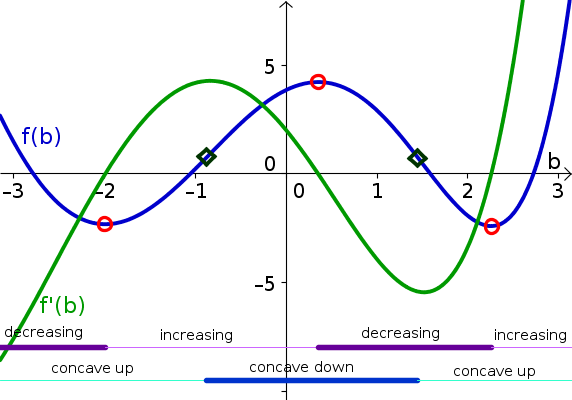
\includegraphics[width=0.4\textwidth]{derivative.png}  % if pdflatex is used, jpg, pdf, and png are permitted
  \caption{Graphing the derivative of f(x).}
  \label{fig:figlabel}
\end{figure}

The derivative of a function, illustrated by the green line in Figure 1, is the slope of the tangent line of f(x). As f(x) reaches a maximum or a minimum point on the graph, the value of f'(x) is 0. When the value of f(x) is decreasing, the value of f'(x) is negative. When f(x) is increasing, f'(x) is positive.
% Repeat as needed

\end{document}

